%
%
%   HONDA
%
%

% 11/14 14:00 nakayama が編集しました。
% 11/16 17:00 nakayama が編集しました。
% 11/24 04:30 nakayama が編集しました。

\documentclass[11pt,b5paper,papersize,dvipdfmx]{jsbook}

\usepackage{vuccaken}
\usepackage{vuccaken2018}
\usepackage{13honda}


% 以下本文
\begin{document}
% \tableofcontents % 目次出力

% - - - - - - - - - - - - - - - - - - - - - - -
\kaishititle{自作CPU}{電気電子工学科4回生}{本田卓}
% - - - - - - - - - - - - - - - - - - - - - - -

%
\section*{はじめに}
一昨年の3月から今年の3月ごろにかけて自作の8 bit CPUをTTLのみで製作しました。
ですから今回はそのCPUの基本仕様、製作中のエピソードなどをまとめました。
かなりマニアックなものですが興味のある方は是非お読みください。

%
\section{CPU解説}

%
\subsection{基本仕様}
\begin{itemize}
    \item bit数 : 8 bit CPU
    \item レジスタ数 : 1個
    \item 動作周波数 : 12 MHz
    \item RISC 命令長 : 16 bit
    \item 1命令16クロック
    \item 命令数 : 18個
\end{itemize}

%
\subsection{基本仕様の解説}
まずこのCPUの基本仕様について解説します。普通CPUの仕様で気になるのはビット数でしょう。最近のパソコンなら32 bitか64 bitのものが使われています。CPUのビット数の定義は詳しく書きませんが、簡単に言えば「そのCPUが一度(1命令)に処理できるデータサイズのこと」です。このCPUでは1命令で8 bitデータを処理できるので8 bit CPUとなります。\par
次にレジスタですが、これはCPU内にある小さなメモリです。CPUの主な処理は「2進数データの演算」と「メインメモリへのデータの格納」です。二つ目のメインメモリへ格納ですが、メインメモリというのは、私たちは「メモリ」とよんでいます、小さければ4 GBくらいで大きければ16 GBくらいのあれです。このメインメモリですが、CPU本体とは離れた場所にあります。ですからCPUとメインメモリが通信するのに時間がかかります。そこで、CPUとメインメモリの間にもう一つCPUから高速にアクセスすることができるメモリを用意します。それがレジスタです(レジスタはCPUの内部に含まれます)。CPUはレジスタに値を格納して、その格納された値をメインメモリへ格納する、という手順を踏みます。普通のCPUならレジスタは複数個備えているのですが、このCPUは回路を単純にするためレジスタを1個しか備えていません。\par
動作周波数はクロックを発生させるICを使っているのでこのICの上限である12 MHzが上限となります。\par
次に命令についてです。CPUの命令は大きく分けてRISCとCISCに分けられます。簡単に説明するとRISCが全命令の命令長が同じ、CISCが命令によって命令長が違うというものです。このCPUではすべての命令が16 bitなのでRISCということになります。次に1命令にかかるクロック数ですが、これはいろいろな資料を参考に考えた結果、16クロックで1命令実行されるような回路になったというだけで、特に深い意味はありません。頑張って設計すればもっと少ないクロック数で1命令を実行できるようになります。簡単で作りやすかったのでこうなりました。そして最後に命令数ですが、これがこのCPU の一番の特徴を表しているといえます。\par
本当に特徴を表しているのはその命令の中身なのですが、とにかく、命令の内容でCPUになにができるかが決まります。詳しくは後で説明しますが、このCPUの命令の特徴を一言でいうと「必要最低限」です。いろいろな命令を実行させる場合はもちろん回路が複雑になります。それが一番嫌だったので、これがあれば最低限のことはできるという程度しか命令を用意していません。次の章で命令について詳しく説明します。\par

\subsection{命令セット}
このCPUが実行できる全命令とその説明をします。まずは説明に使われる用語の説明を行います。
\begin{itemize}
    \item A:レジスタのこと。複数あればレジスタA,レジスタB, ...となります。今回はAレジスタしかないのでAしか出てきません。
    \item 機械語:2進数(0,1)で表現された実際にCPUが読み取る命令のこと。
    \item アセンブラ:機械語の1命令をわかりやすいように2進数から文字に変換したもの。
    \item IM(Immediate data):機械語命令の後半部分の値のこと(前半部分はオペコード)。
    \item プログラムカウンタ(PC):メインメモリの中で実際に実行される命令が格納されているアドレス(番地)を示す値。通常1命令実行されるたびインクリメントされる。
\end{itemize}
次に命令の例を表\ref{tbl:meex}に、全命令とその説明をまとめた命令表を表\ref{tbl:me}に示します。

\begin{table}[htb]
    \centering
    \caption{命令の例}
    \begin{tabular}{lcc}
        \hline
        &{\small オペコード} &{\small IM}\\\hline
        {\small アセンブリ}&{\small LDIM}&{\small 3}\\
        {\small 機械語 }&{\small 0101\ 0000}&{\small 0000\ 0011}\\
        {\small 意味 }& \multicolumn{2}{c}{{\small Aレジスタに3を格納する}}  \\\hline
    \end{tabular}
    \label{tbl:meex}
\end{table}
%
\renewcommand{\arraystretch}{1.5}
\begin{table}[htb]\small
    \centering
    \caption{命令表}
    \begin{tabular}{lcll}%
        \hline
        \shortstack{\\命令\\{\scriptsize アセンブラ表記}} & \shortstack{\\機械語\\{\scriptsize (16進数)}} & \shortstack{説明\\\,} & \shortstack{式\\\,} \\
        \hline
        LDIM	&50	&{\scriptsize \parbox{23zw}{IMデータをAレジスタにロードする}}	                                         &A = IM\\
        ADDIM	&91	&{\scriptsize \parbox{23zw}{Aレジスタの値にIMの値を足したものをAレジスタに格納する}}	                       &A = A + IM\\
        SUBIM	&62	&{\scriptsize \parbox{23zw}{Aレジスタの値にIMの値を引いたものをAレジスタに格納する}}	                       &A = A $-$ IM\\
        ANDIM	&D3	&{\scriptsize \parbox{23zw}{Aレジスタの値とIMの値のANDをとったものをAレジスタに格納する}}	               &A = A AND IM\\
        NOTIM	&3	&{\scriptsize \parbox{23zw}{Aレジスタの値とIMの値のNOTをとったものをAレジスタに格納する}}	               &A = A AND IM\\
        ORIM	&74	&{\scriptsize \parbox{23zw}{Aレジスタの値とIMの値のORをとったものをAレジスタに格納する}}	                   &A = A AND IM\\
        LDMEM	&55	&{\scriptsize \parbox{23zw}{AレジスタにメインメモリのIM番地の値を格納する}}	                          &A = [IM]\\
        ADDMEM	&96	&{\scriptsize \parbox{23zw}{Aレジスタの値にメインメモリのIM番地の値を足したものをAレジスタに格納する}}	    &A =  A + [IM]\\
        SUBMEM	&67	&{\scriptsize \parbox{23zw}{Aレジスタの値にメインメモリのIM番地の値を引いたものをAレジスタに格納する}}	    &A = A $-$ [IM]\\
        ANDMEM	&D8	&{\scriptsize \parbox{23zw}{Aレジスタの値とメインメモリのIM番地の値のANDをとったものをAレジスタに格納する}}	&A = A AND [IM]\\
        NOTMEM	&8	&{\scriptsize \parbox{23zw}{Aレジスタの値とメインメモリのIM番地の値のNOTをとったものをAレジスタに格納する}}	&A = A NOT [IM]\\
        ORMEM	&79	&{\scriptsize \parbox{23zw}{Aレジスタの値とメインメモリのIM番地の値のORをとったものをAレジスタに格納する}}	&A = A OR [IM]\\
        JMP	    &5A	&{\scriptsize \parbox{23zw}{プログラムカウンタの値をIMに変更する}}	                                 &PC = IM\\
        JNC	    &5B	&{\scriptsize \parbox{23zw}{キャリーフラグが1の場合プログラムカウンタをIMにする}}	                      &PC = IM (CF = 1)\\
        JNZ	    &5C	&{\scriptsize \parbox{23zw}{ゼロフラグが1の場合プログラムカウンタをIMにする}}	                          &PC = IM (ZF = 1)\\
        STR	    &D	&{\scriptsize \parbox{23zw}{Aレジスタの値をメインメモリのIM番地に格納する}}	&[IM] = A\\
        IN	    &5E	&{\scriptsize \parbox{23zw}{INポートの値をAレジスタに格納する}}	&A = IN\\
        OUT	    &F	&{\scriptsize \parbox{23zw}{Aレジスタの値をOUTポートに出力する}}	&OUT = A\\
        \hline
    \end{tabular}
    \label{tbl:me}
\end{table}
\renewcommand{\arraystretch}{1}

% \begin{figure}[H]
%     \centering
%         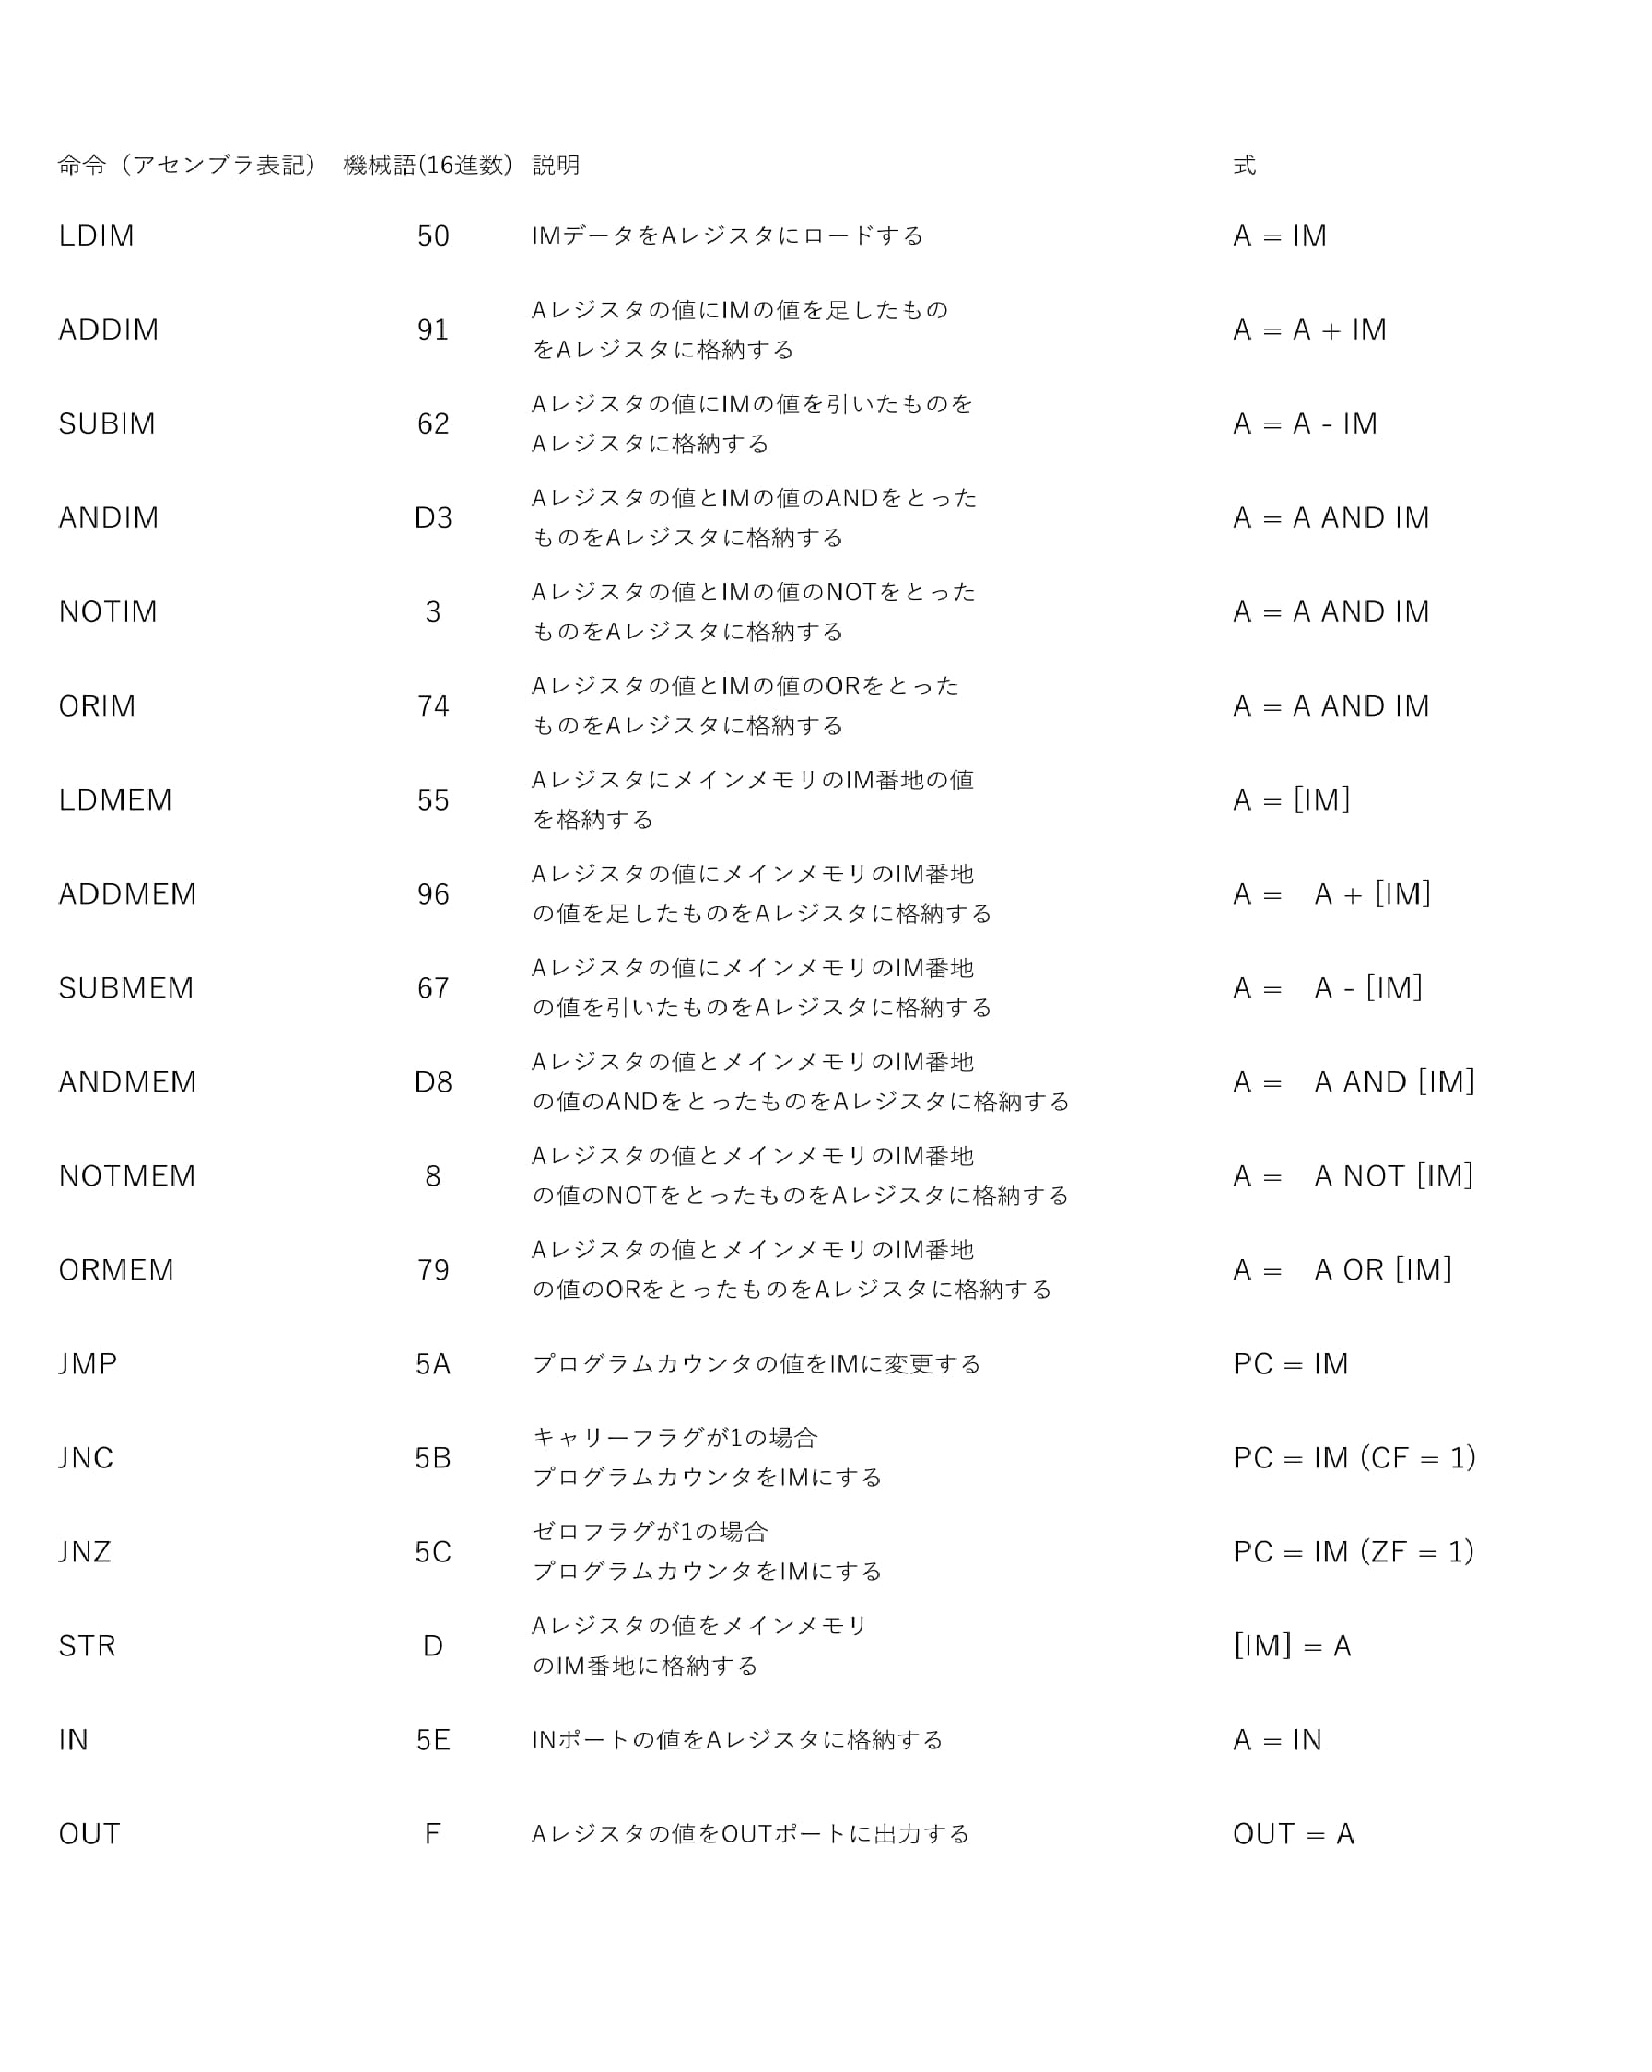
\includegraphics[width=11cm]{honda/img/op_list-1.jpg}
%         \caption{命令表}
%         \label{fig:meirei}
% \end{figure}

\clearpage
%
\subsection{サンプルコード}
\hndcodecaption{$3 \times 5$の計算}
\begin{hndcode}
    LDIM 0
    STR 0  
    STR 1
bbb:LDIM 5
    SUBMEM 1
    JNZ aaa
    LDMEM 0
    ADDIM 3
    STR 0
    LDMEM 1
    ADDIM 1
    STR 1
    JMP bbb
aaa:LDMEM 0
    OUT
ccc:JMP ccc
\end{hndcode}

\paragraph{解説}
最初のLDIM 0, STR 0, STR 1でメインメモリの0番地と1番地に0を格納します。
次にLDIM 5, SUBMEM 1で5からメインメモリの1番地の値を引きます。
はじめは0が格納されているので答えは5が返ってきます。
ここで答えが0だった場合次のJNZ aaaに引っかかり
aaaアドレス(プログラム中のaaa: LDMEM 0)にジャンプしますが、
今回は5なのでそのまま次の命令に行きます。LDMEM 0, ADDIM 3, STR 0で
メインメモリの0番地の値をAレジスタに持ってきて、それに3を足してまた0番地に戻します。
次のLDMEM 1, ADDIM 1, STR 1で同様に1番地の値を持ってきて1足してまた1番地に戻します。
ここでJMP bbbによりbbbの地点に戻るのでこれまでの命令が繰り返されるのですが、1番地の値が1足されているので最初のLDIM 5, SUBMEM 1, JNZ aaaのとろこが$5-1=4$となります。これでも0ではないのでJNZでaaaにはジャンプしないのですが、これをあと4回繰り返すと$5-5$となりJNZ aaaが実行されてaaa地点の実行へ移ります。そこからはLDMEM 0で0番地の値を呼び出してOUTでOUTポートに出力(Aレジスタの値を人が見えるようにLEDで表示)します。JMP cccはその場無限ループなのでこれ以上もうCPUは何もしません。\par

\hndcodecaption{1から10まで足し算}
\begin{hndcode}
    LDIM 0
    STR 0
    LDIM 1
    STR 1
    LDIM 10
    STR 2
bbb:LDMEM 0
    ADDMEM 1
    STR 0
    LDMEM 1
    ADDIM 1
    STR 1
    LDMEM 2
    SUBIM 1
    JNZ aaa
    STR 2
    JMP bbb
aaa:LDMEM 0
    OUT
ccc:JMP ccc
\end{hndcode}

\paragraph{解説}
前の$3\times5$のプログラムで詳しく説明したので今回は少しざっくりと説明します。
最初のLDIM 0, STR 0,LDIM 1 STR 1, LDIM 10, STR 2でメインメモリの0番地に0、
1番地に1、2番地に10を格納します。
つぎにLDMEM 0, ADDMEM 1, STR 0でメインメモリ0番地の値と1番地の値を足します。
次のLDMEM 1, ADDIM 1, STR 1で1番地の値を1増やします。
これで次は0番地の値に2が足されます。最後にLDMEM 3, SUBIM 1, STR 3で3番地の値から1引きます。
3番地にはもともと10が入っており、引き算の答えが0になったとき(10ループしたとき)JNZ cccでループを抜けて0番地の値をOUTで出力します。

%
\section{製作小話}
%
\subsection{製作に至った経緯}
もともとサークル活動として電子工作、マイコンを使ったプログラミングをしていました。
そんな中で「マイコンの中身ってどうなっているんだろう」という疑問を持っていましたが、同時に「ものすごい複雑な構造をしていて、簡単にわかるものではない」とも思っていました。
ですが、ある日偶然「論理回路だけで電卓を作る」というサイトを見つけました。
そこにはとても分かりやすく論理回路で計算機を作る方法が解説されており、論理回路の基礎しか知らない僕でも簡単に理解することができました。
これをきっかけに「もしかしたらCPUの構造も論理回路だけで理解できるかもしれない」と思いました。そこから名著「CPUの創り方」を読んだり、
自分で勉強したりしてある程度CPUを理解することができました。ですが、この時はまだCPU自作をしたいとは思っていても、できるとは思えず行動はしていませんでした。
そんなとき、詳しくは説明できませんが、とんでもないミラクルが起き、回路のスペシャリストの方と知り合うことができ、僕がCPUを自作したいと話すと、「ぜひ一緒に作りましょう」という流れになり、その結果CPUを作ることになりました。
そこから一年かかりましたが無事CPUを完成させることができました。かなり運がよかったと思います。

%
\subsection{はんだ挫折}
今完成しているCPUは外注基板でできていますが最初はユニバーサル基板でジャンパー配線の手はんだで作ろうとしていました。書き込み回路だけは手はんだで作りましたが(僕ではなくはんだ付けが得意な友達がやってくれました)あまりの面倒くささに手はんだは断念して外注基板に変更することになりました。下図が実際にはんだ付けされた基板です。

\begin{figure}[H]
    \centering
    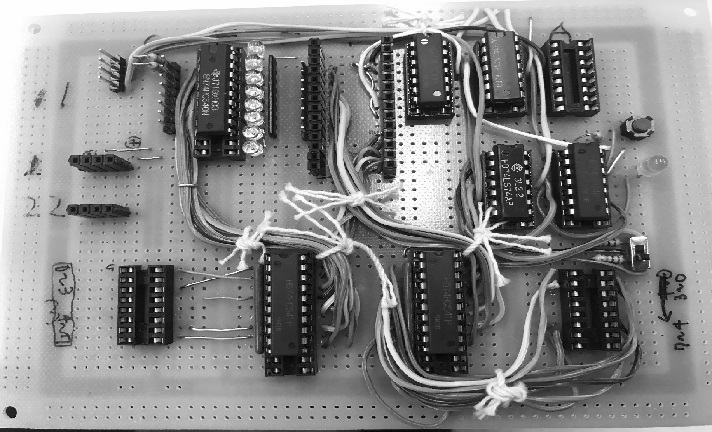
\includegraphics[width=4.4cm]{honda/img/monokuro_kairo.png}
    \caption{ユニバーサル基盤にはんだ付けした回路}
    \label{fig:kairo-of-handa}
\end{figure}

%
\subsection{お世話になった資料}
このCPUを作るまでにいろいろな資料にお世話になりました。その中でも特に役に立った資料(本、サイトなど)を紹介します。\par
\begin{itemize}
    \item 電卓製作サイト\par
        \url{http://www7b.biglobe.ne.jp/~yizawa/logic2/chap1/index.html}\par
        先ほども書いたように僕がCPUを作ることになったきっかけです。普通「CPUは論理回路だけでできている」と言われても想像がつきません。ですが、このサイトの丁寧な解説で自分が思っているほどCPUの内部回路は難しくないのかもしれないと思えるようになりました。
    \item CPUの創り方\par
    有名なやつです。TTLを10個だけでCPUを自作するという本です。これがCPUなのかというほど簡単なCPUを作りますが、基本構造は変わらないのでこれを理解できればCPUの基本は理解できます。いきなり最新の複雑なCPUを理解できるわけがないので、最初はこの本のような最小構造のCPUを勉強するのが一番いいと思います(趣味で勉強するなら)。
    \begin{figure}[H]
        \centering
        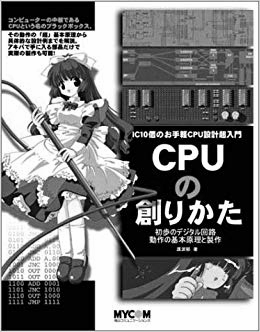
\includegraphics[width=5.5cm]{honda/img/51ATDABNHEL.png}
        \caption{CPUの創り方}
        \label{fig:how-to-create-cpu}
    \end{figure}
    \item がたろうさんのサイト\par
    \url{http://diode.matrix.jp/}\par
    自作CPUを作るおじいさんのサイトです。この人が作ったCPUの回路を参考に今回のCPUを製作しました。CPUだけでなく、独自のコンパイラ、OSなどほとんどのものを自作しています。この人のまねをしたといっても間違いではないです。
\end{itemize}

%
\subsection{こんなことしないでシミュレーションソフトを使いましょう}
最後にこれを見て少しでもCPUに興味を持たれた方がいるなら一つアドバイスですが、はんだ付けして実物が欲しい!などと思わなければ、論理回路シミュレータという素晴らしいものがあるのでそちらを使いましょう。フリーソフトでだれでも簡単に使えます。僕が使っているのはLogisimというソフトです。作った回路が実際にCPUとして動作するか確認として使っていましたが、とても便利でした。正直途中から「シミュレータで動いたんだからもうはんだ付けしなくてもいいか」とも思っていました。変更点があれば一瞬で変更できるし、コピぺできるし、ほかの人が作った部品流用できるし、完璧です。ネットにほかの人がlogisimで作ったCPUが上がっているのでそれを参考にすることもできます。「CPUの創り方」のCPUなんてすぐ作れます。まあ、実物は思い出になりますし、いいところもあります。(でももう作りません)

% 参考文献
\sanko
\begin{enumerate}
\item 渡波 郁, CPUの創り方, 毎日コミュニケーションズ.
\end{enumerate}


\end{document}
%
% ファイトだよ!
% お疲れ様なのだ!
%